\documentclass[prez_tpt]{subfiles}
\begin{document}


%========================================================================
\section{Studying physiological signals}
%========================================================================
%------------------------------------------------------------------------
\subsection{Motivations}
%------------------------------------------------------------------------
%
\begin{frame}{Dictionary Learning \citeconfright{Olshausen1997}{Vision Research}}
\begin{columns}[c]
    \column{.4\textwidth}
        Dictionary learning learns a set of atoms (patterns) to sparsely
        reconstruct a signal,\\[2em]
        \textbf{Goal:}\\[1em]
        \begin{itemize}\itemsep1em
            \item Feature extraction,
            \item Signal exploration.
        \end{itemize}
    \column{.6\textwidth}
    \centering
    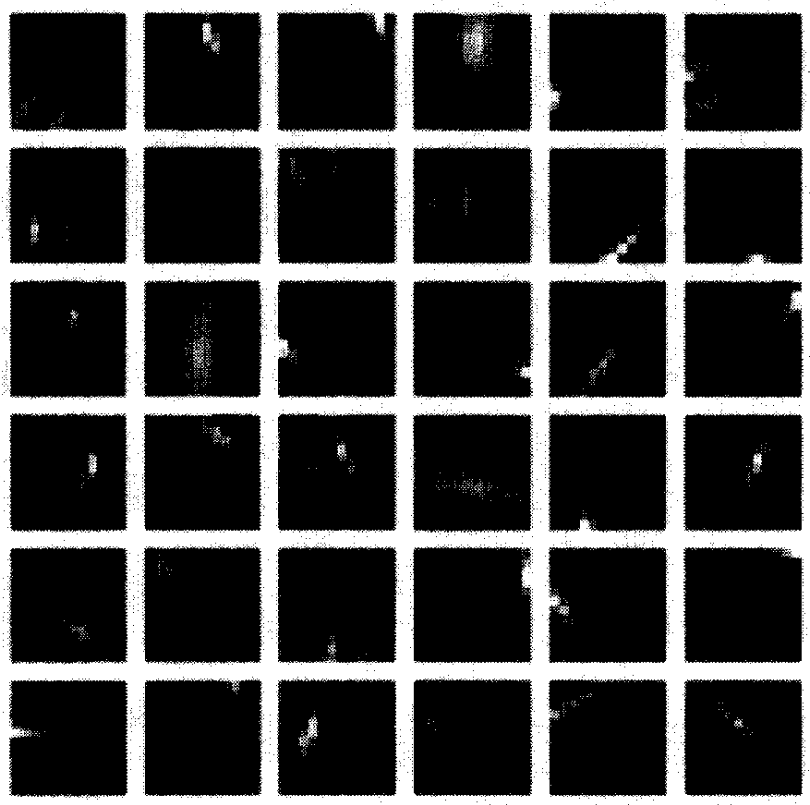
\includegraphics[width=.7\textwidth]{olshausen}\\[.5em]
    Patches learned with natural images\\ in \citealt{Olshausen1997}.
\end{columns}
\end{frame}

\begin{frame}{Convolutional Dictionary Learning \citeconfright{Grosse2007}{UAI}}

{\centering 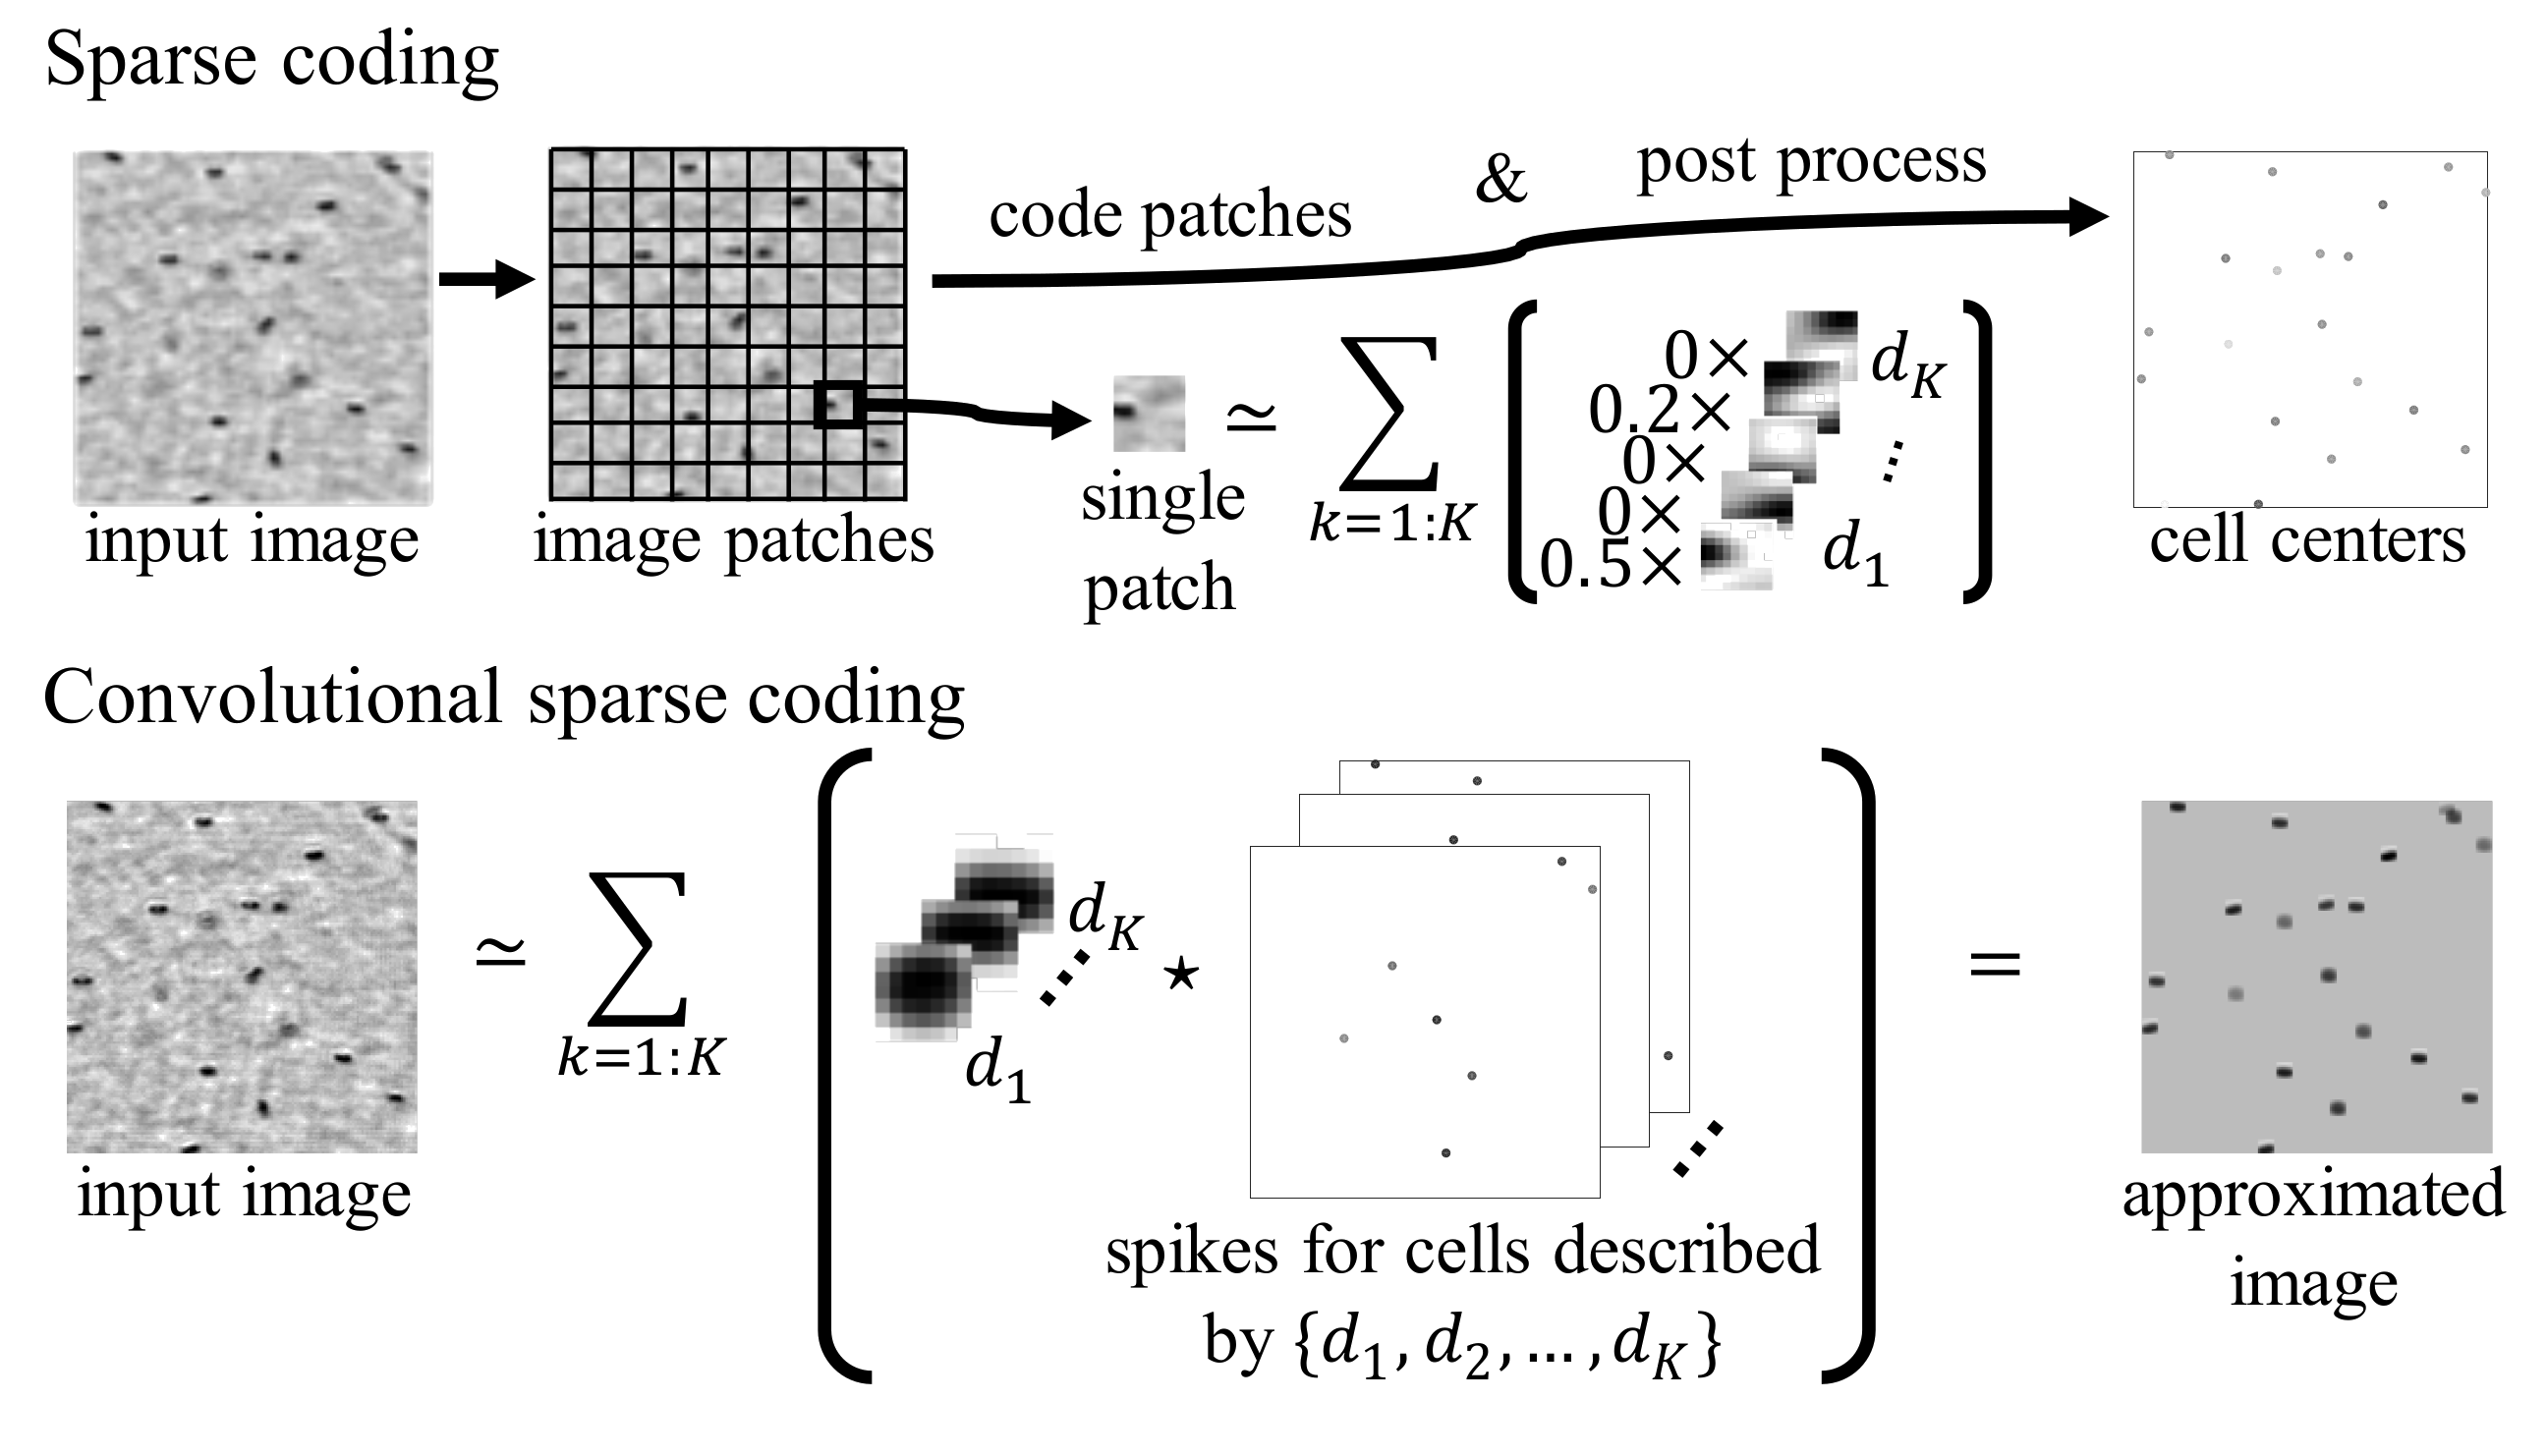
\includegraphics[width=.7\textwidth]{blood_cell_images}\\(Credit to \citep{Yellin2017})\\[.5em]}

{\color{red} Convolutional} Dictionary Learning learns a set of {\color{red} shift-invariant} atoms to sparsely reconstruct a signal,
\begin{columns}[T]
    \column{.3\textwidth}
    \begin{itemize}
        \item Improve sparsity
    \end{itemize}
    \column{.3\textwidth}
    \begin{itemize}
        \item Not all patches are encoded
    \end{itemize}
    \column{.3\textwidth}
    \begin{itemize}
        \item Sharper atoms
    \end{itemize}
\end{columns}
\end{frame}

\begin{frame}[t]{Application fields}

{
\centering
\vskip1em
\only<1>{
    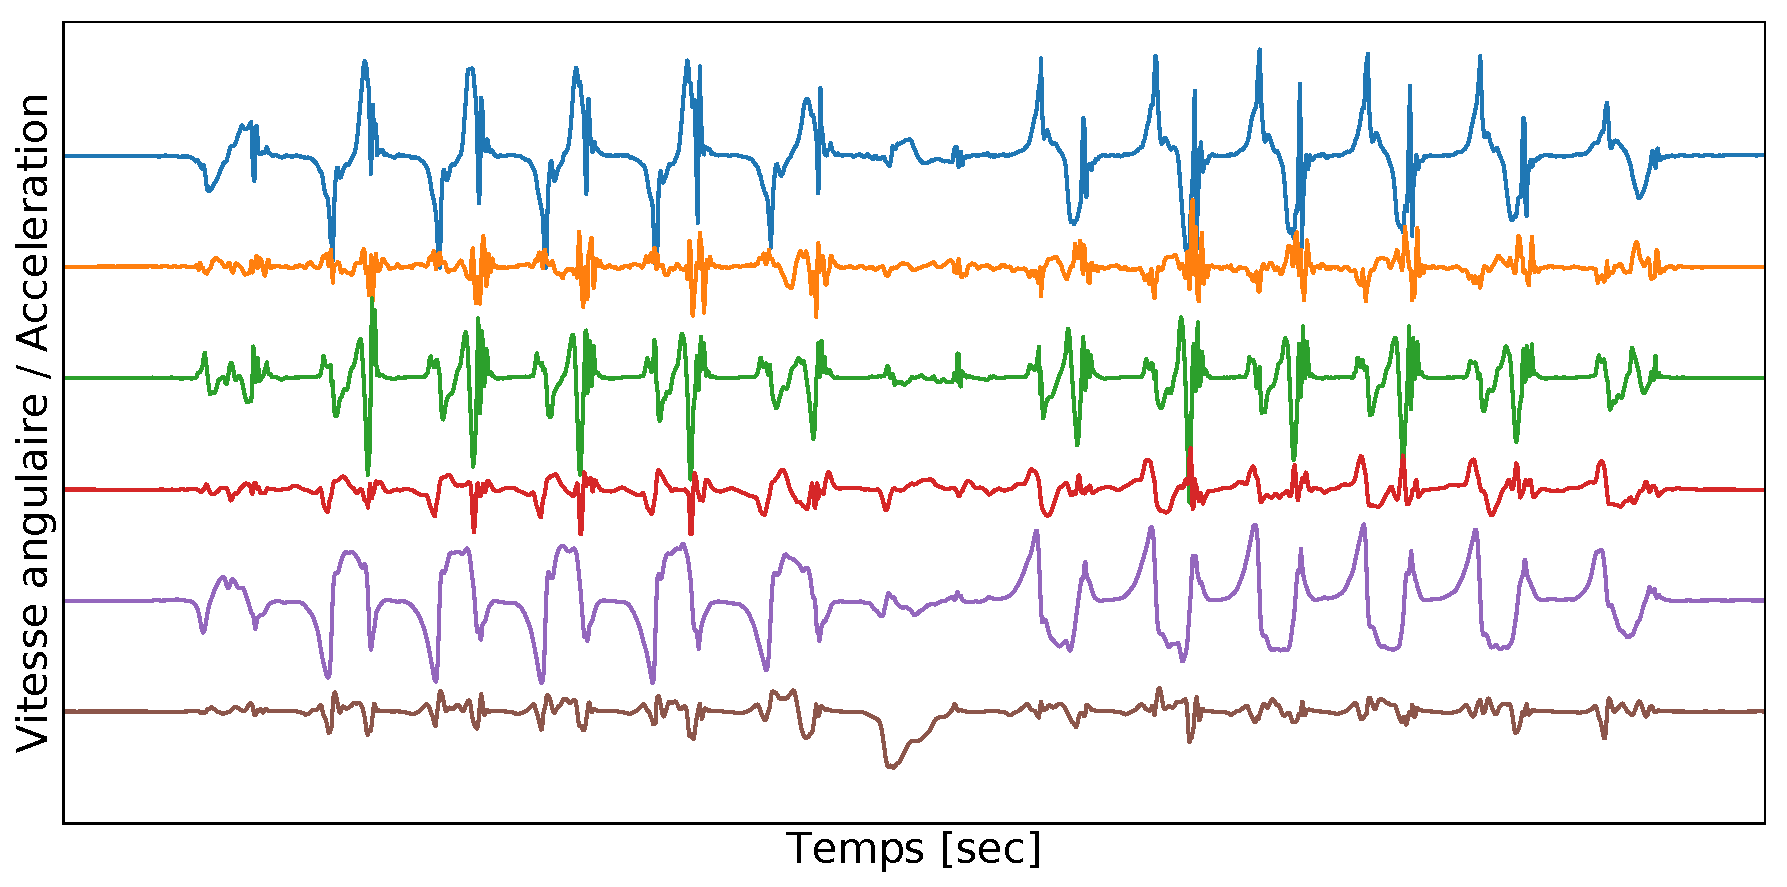
\includegraphics[height=.4\textheight]{accelero}\\%

    \citeconf{Oudre2018}{Sensors}\\
    {\usebeamercolor[bg]{normal text}.}\\
}
\only<2>{
    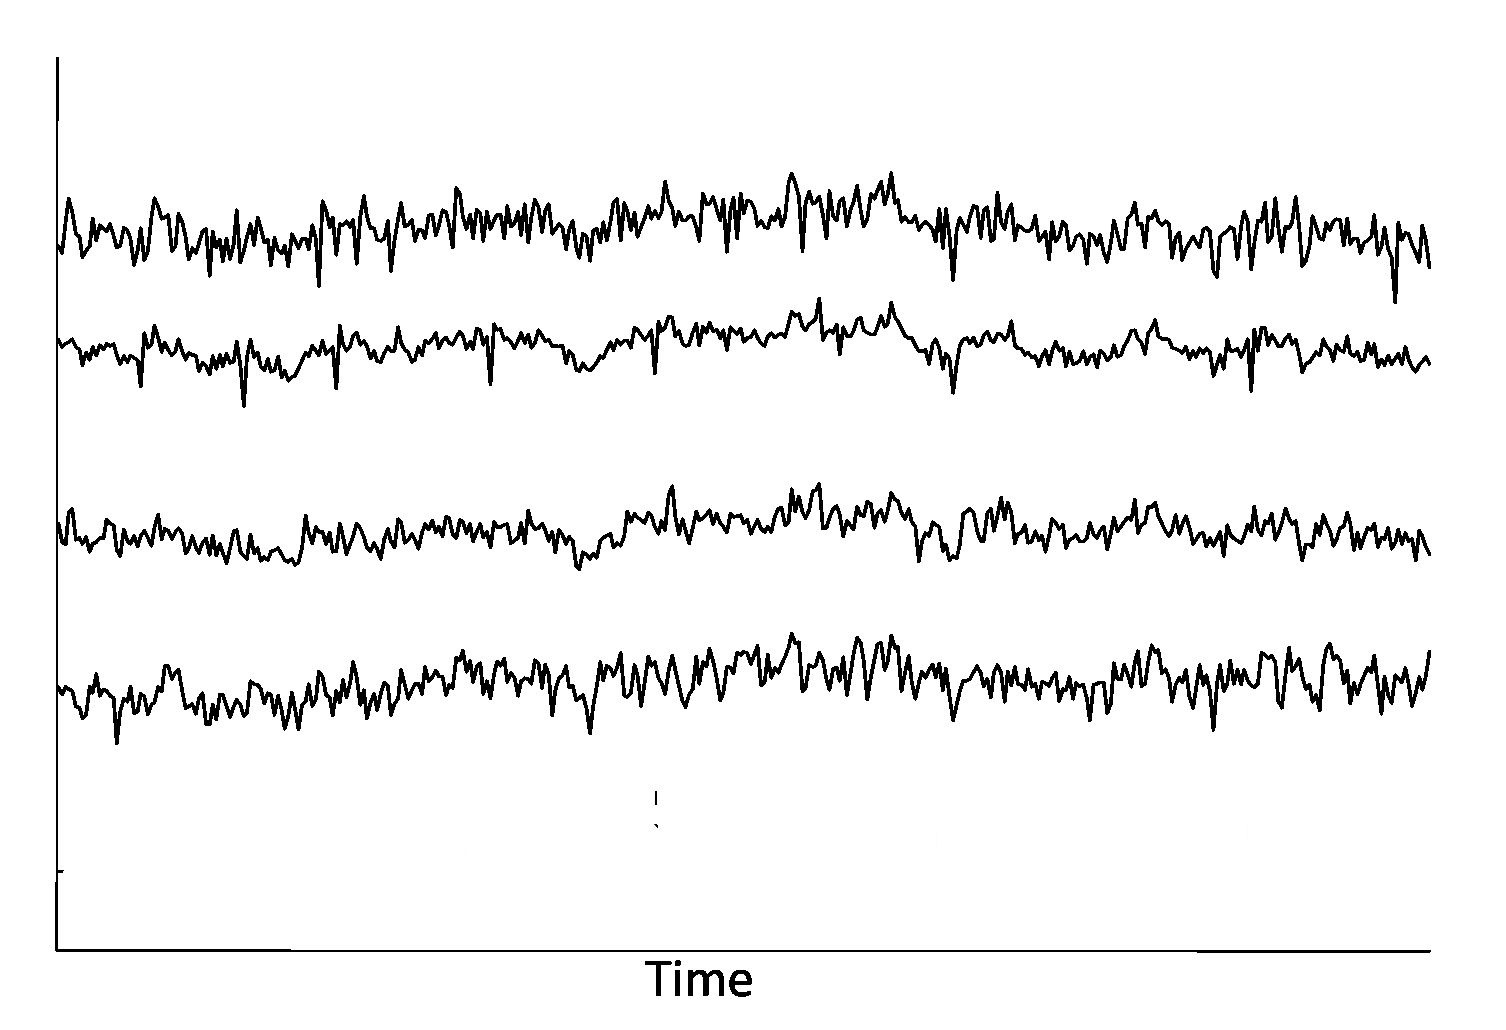
\includegraphics[height=.4\textheight]{multivariate_eeg}\\%

    \citeconf{Dupre2018}{NeurIPS}\\
    {\usebeamercolor[bg]{normal text}.}\\
}
\only<3>{
    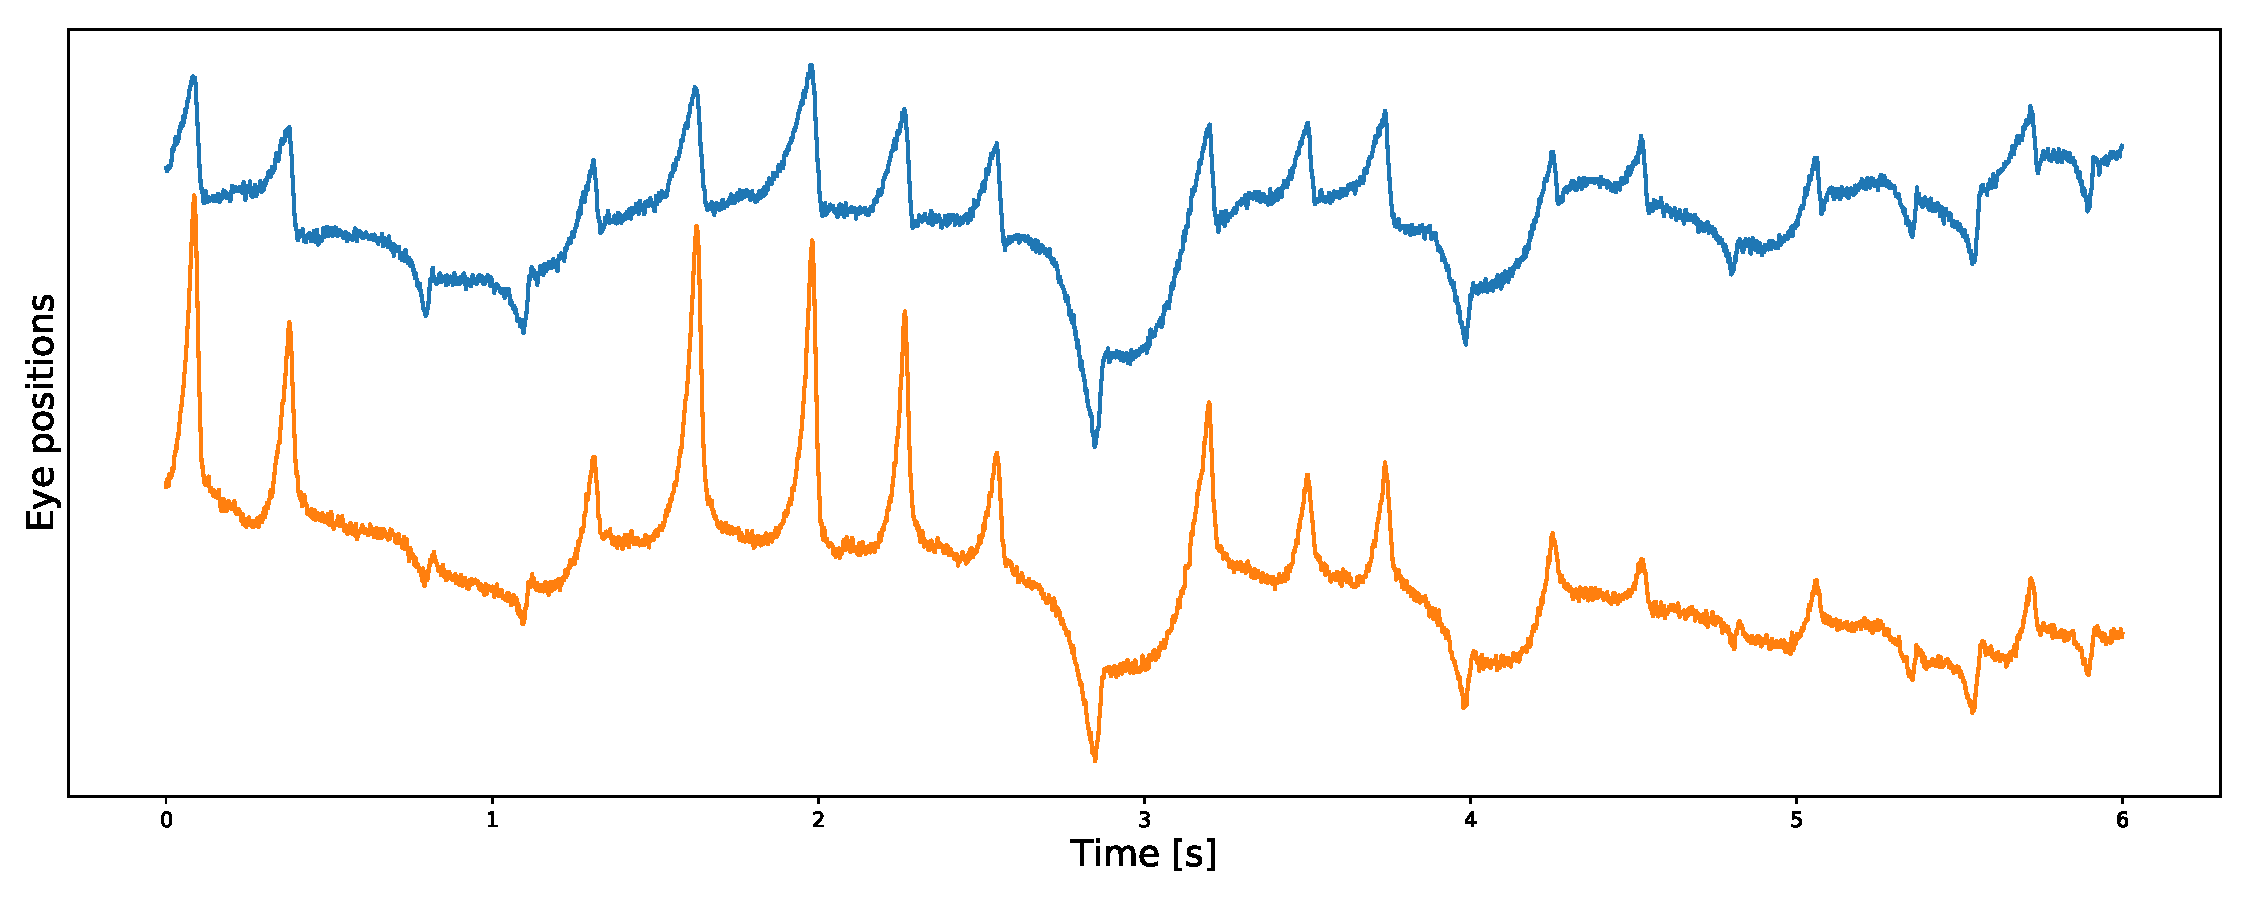
\includegraphics[height=.4\textheight]{oculo}\\%

    \citeconf{Robert2016}{preprint}\\
    {\usebeamercolor[bg]{normal text}.}\\
}
\only<4>{
    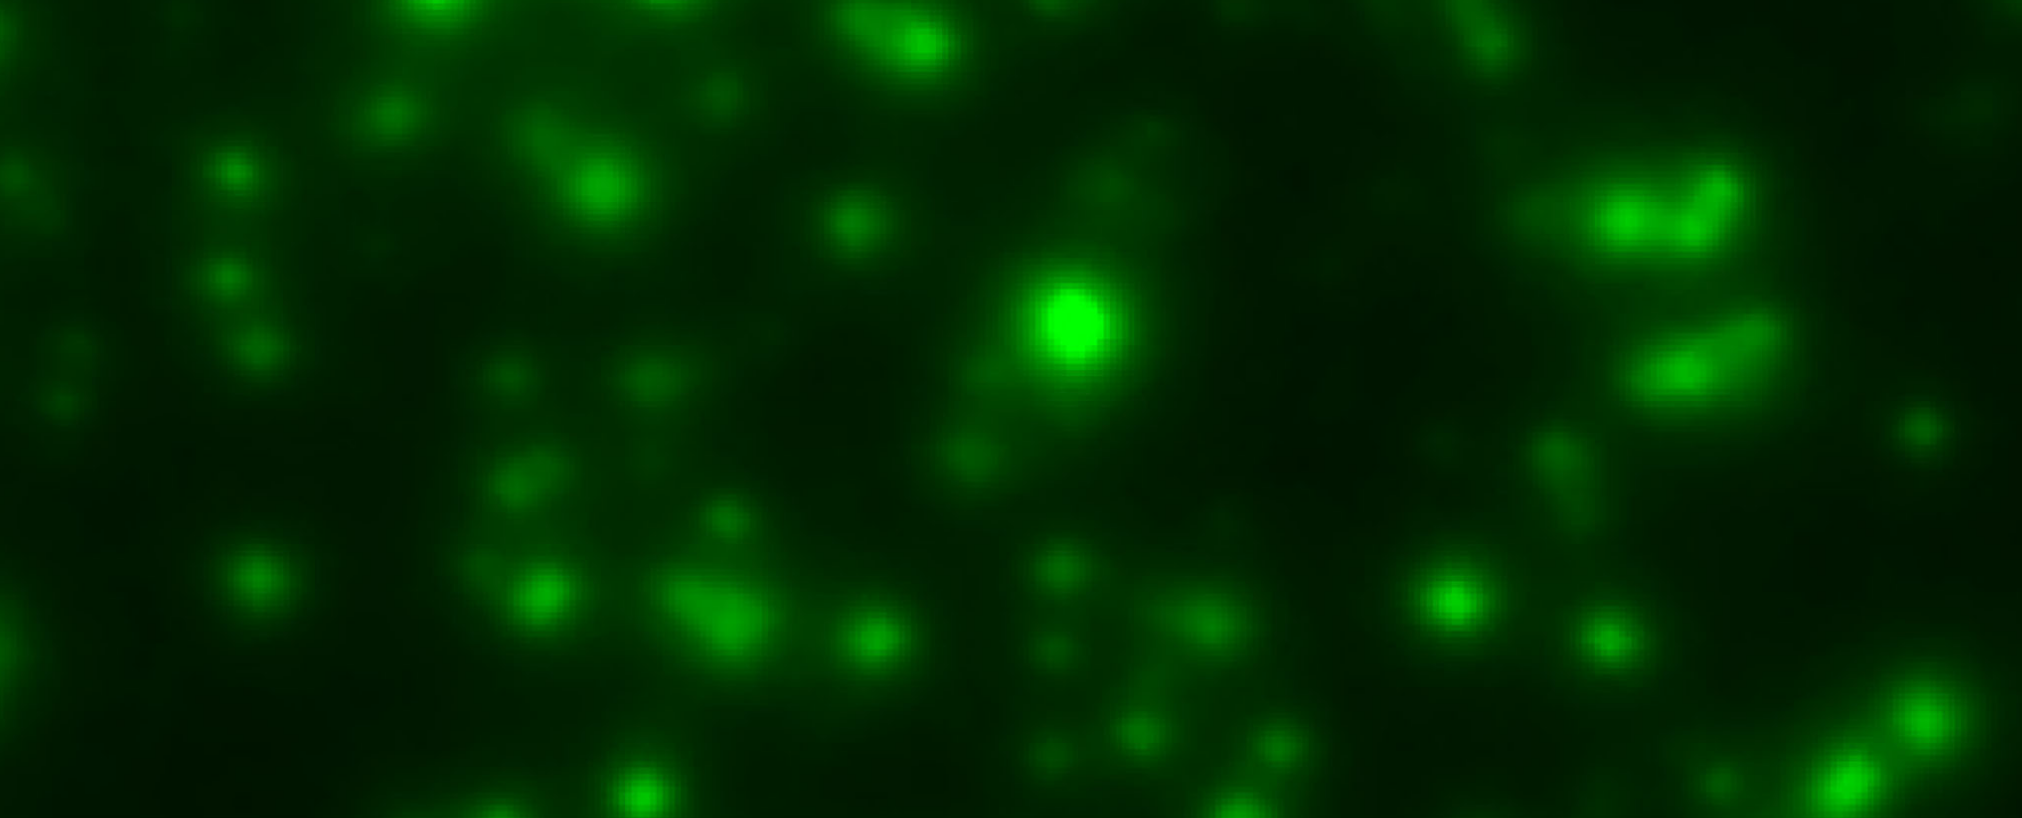
\includegraphics[height=.4\textheight]{fluospot}\\%
    
    [{\color{linkcolor}del Aguila Pla et al. 2018, IEEE TSP};
     \citealt{Yellin2017}{\color{linkcolor}, ISBI}]\\
     {\usebeamercolor[bg]{normal text}.}\\
}
\only<5>{
    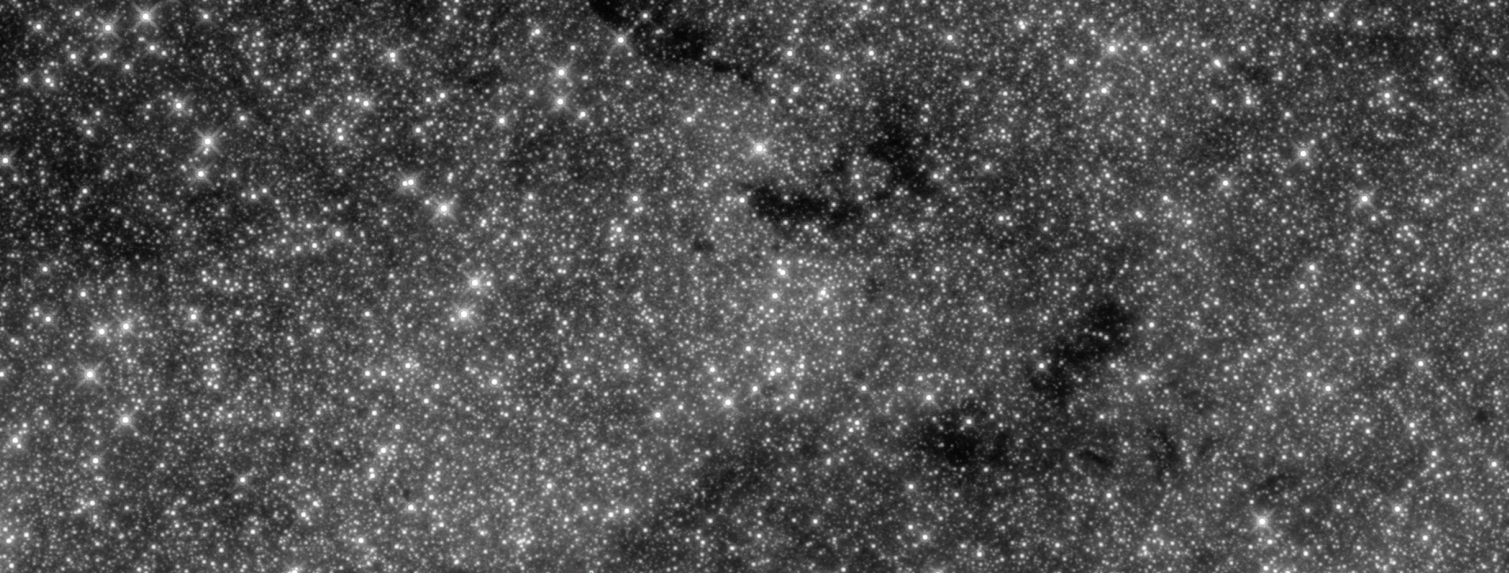
\includegraphics[height=.4\textheight]{milky}\\%
    
    [{\color{linkcolor}del Aguila Pla et al. 2018, ICASSP};\\
    \citealt{Beckouche2013}{\color{linkcolor}, Astronomy \& Astrophysics}]\\
}
}
\begin{itemize}[<+->]
    \item  Detecting steps in human walk recordings to predict elderly falls.
    \item  Exploring neurological signals from ECG and MEG,
    \item  Classifying pathological eye movements form oculomotor signals.
    \item  Counting cells in biological images.
    \item Counting stars and galaxies in telescope images
\end{itemize}
    

\end{frame}


\begin{frame}[t]{Challenges of Convolutional Dictionary Learning}
    \begin{itemize}\itemsep1em
        \item \textbf{Computational:} how to scale with large signals,
        \begin{itemize}
            \item {\only<2>{\color{red}}by exploiting the structure of the dictionary.}\\
            \visible<2>{[\citealt{Moreau2017}{\color{linkcolor}, ICLR}]}
            \item {\only<2>{\color{red}}by parallellization.}\\
            \visible<2>{[\citealt{Moreau2018}{\color{linkcolor}, ICML};
                         \citealt{Moreau2019}{\color{linkcolor}, preprint}]}
        \end{itemize}
        \item \textbf{Modelization:} how to incorporate prior knowledge,
        \begin{itemize}
            \item on the activations.\\[1em]
            \item {\only<2>{\color{red}}on the patterns.}\\
            \visible<2>{[\citealt{Dupre2018}{\color{linkcolor}, NeurIPS}]}
        \end{itemize}
        \item \textbf{Evaluation:} how to evaluate the quality of the learned patterns.
        \item \textbf{Theoretical:} pattern recovery.
    \end{itemize}
\end{frame}

\begin{frame}%{Outline}
\vfill
\newlength{\sepbox}
\setlength{\sepbox}{.5em}
\centering
\begin{beamercolorbox}[sep=8pt,center,shadow=true,rounded=true]{title}
    \usebeamerfont{title}\color{darkblue!80}\nameref{sec:cdl}%
\end{beamercolorbox}
\vskip\sepbox
\begin{beamercolorbox}[sep=8pt,center,shadow=true,rounded=true]{title}
\usebeamerfont{title}\color{darkblue!80}\nameref{sec:lista}%
\end{beamercolorbox}
\vskip\sepbox
\begin{beamercolorbox}[sep=8pt,center,shadow=true,rounded=true]{title}
\usebeamerfont{title}\color{darkblue!80}\nameref{sec:lgcd}%
\end{beamercolorbox}
\vskip\sepbox
\begin{beamercolorbox}[sep=8pt,center,shadow=true,rounded=true]{title}
\usebeamerfont{title}\color{darkblue!80}\nameref{sec:multicsc}%
\end{beamercolorbox}
\vfill

\end{frame}


%------------------------------------------------------------------------
\section{Convolutional Dictionary Learning}
\label{sec:cdl}
%------------------------------------------------------------------------

\parttitleframe{Grosse2007}


\begin{frame}{Extracting shift invariant patterns}
\textbf{Key idea}: decouple the localization of the patterns and their shape
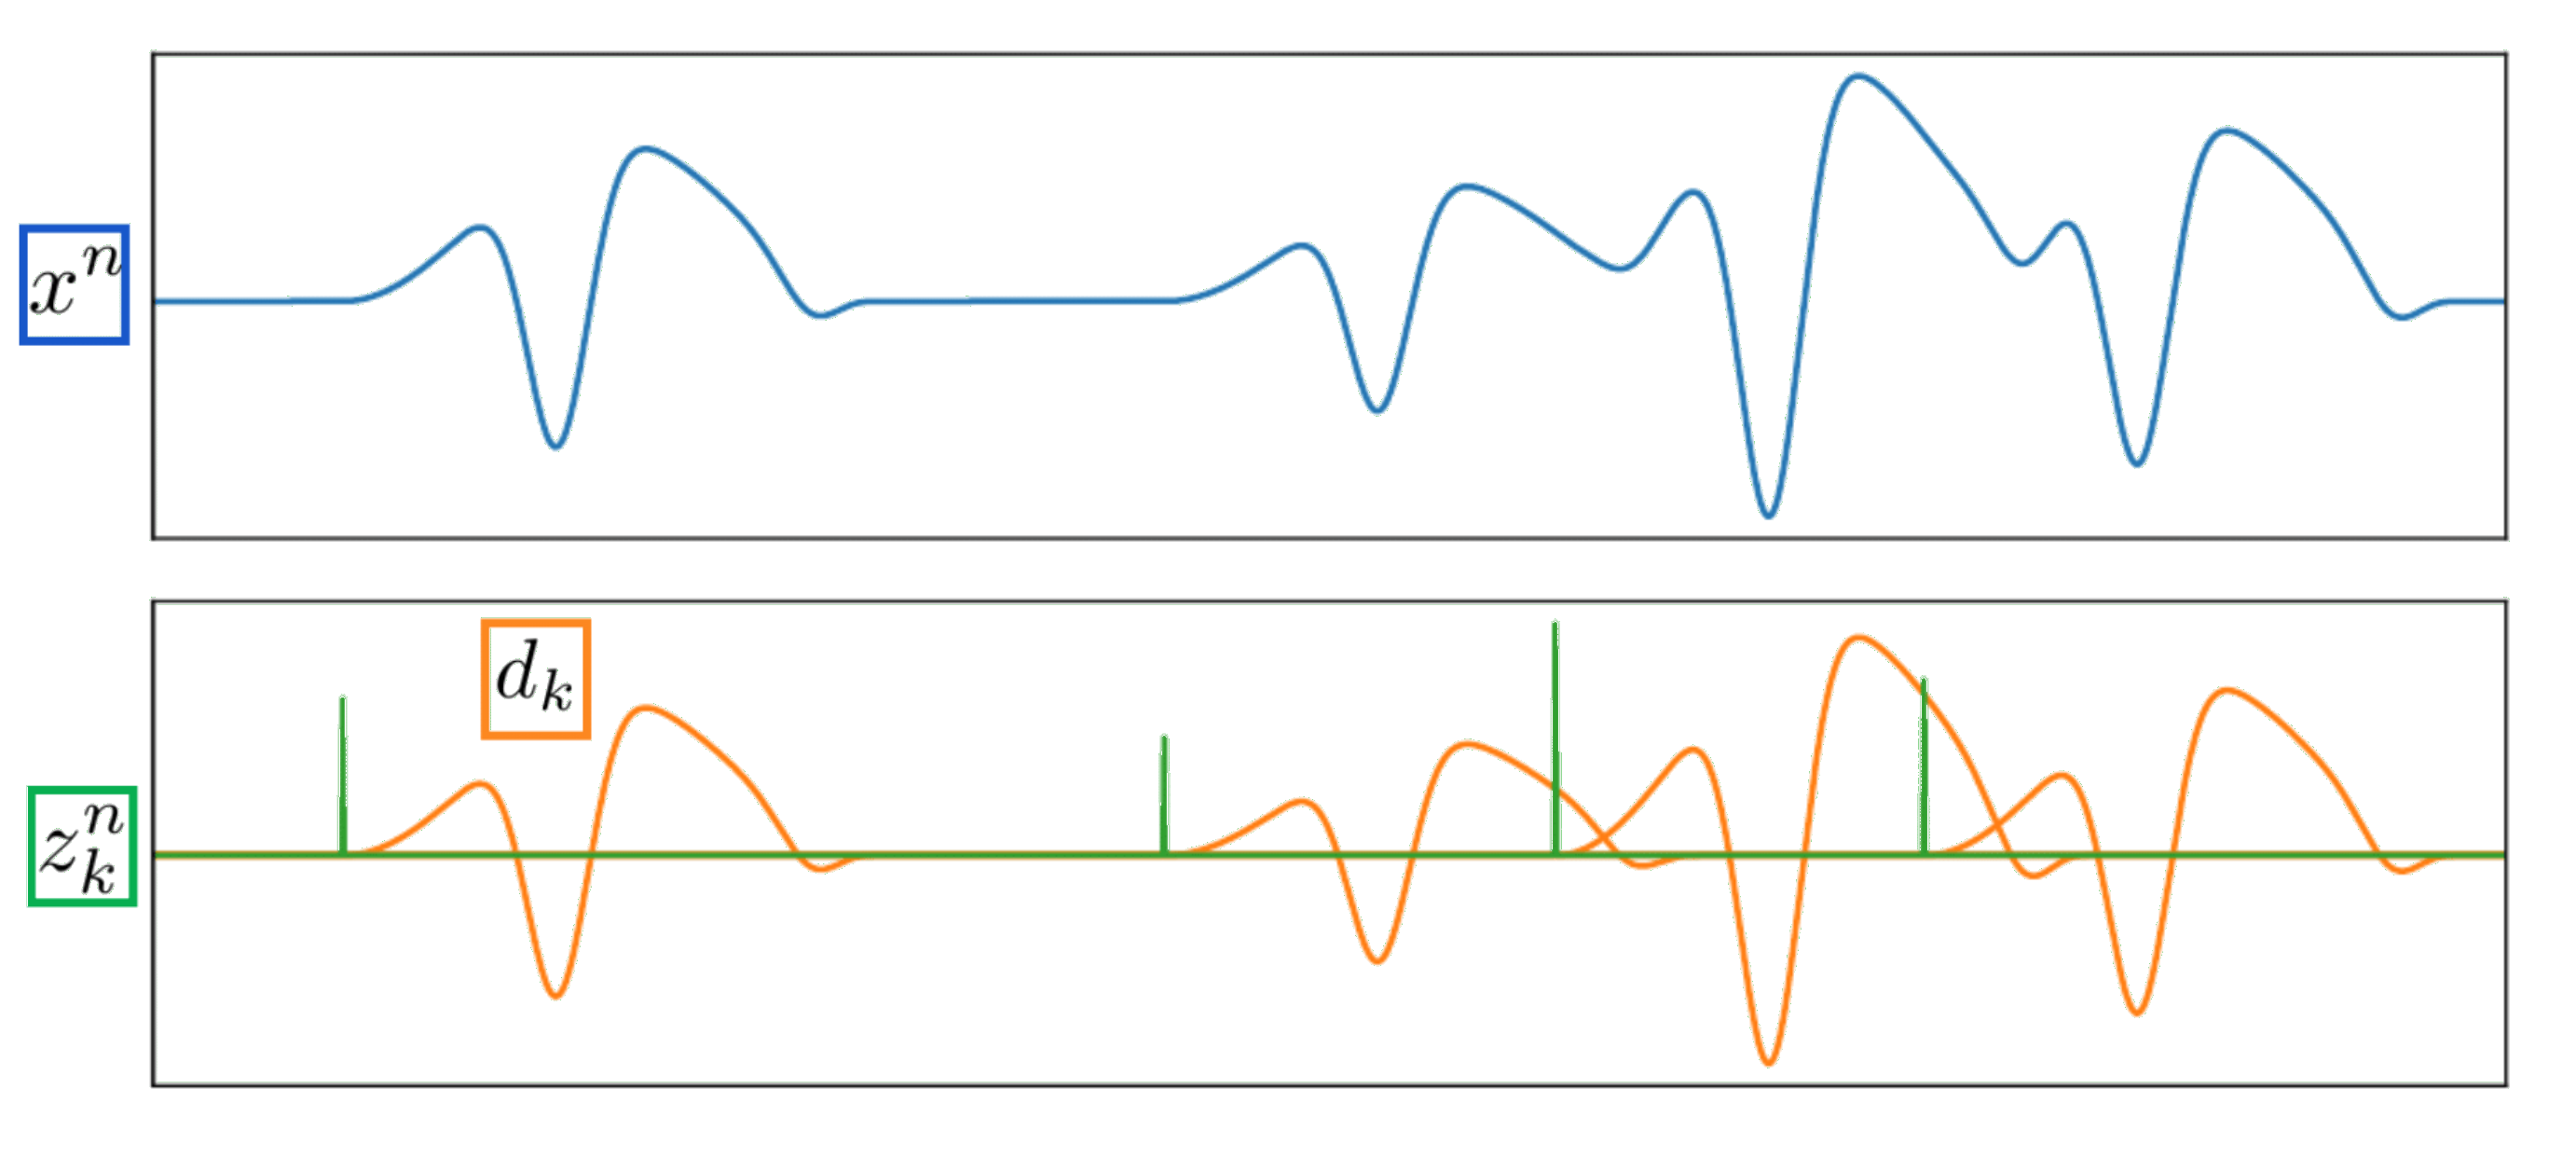
\includegraphics[width=\textwidth]{csc_explain_color.png}
\only<2>{
    \vskip-2em
    \begin{columns}[T]
        \column{.3\textwidth}\vskip2em\centering\textbf{Convolutional\\Representation:} %
        \column{.7\textwidth}\centering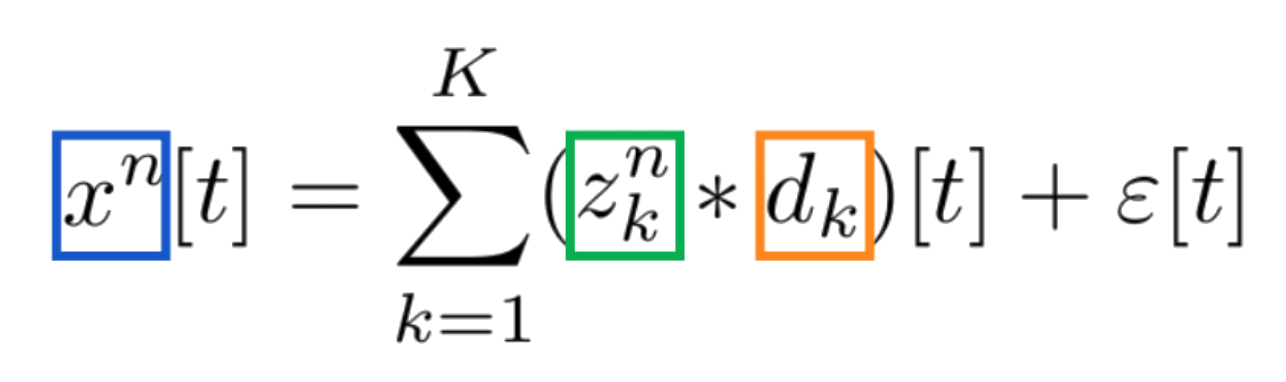
\includegraphics[width=.7\textwidth]{csc_explain_eq_color}
    \end{columns}
}
\uncover<3>{
    \vskip-2em
    \begin{columns}[T]
        \column{.3\textwidth}\vskip2em\centering\textbf{Convolutional Dictionary Learning:} %
        \column{.7\textwidth}\vskip-.5em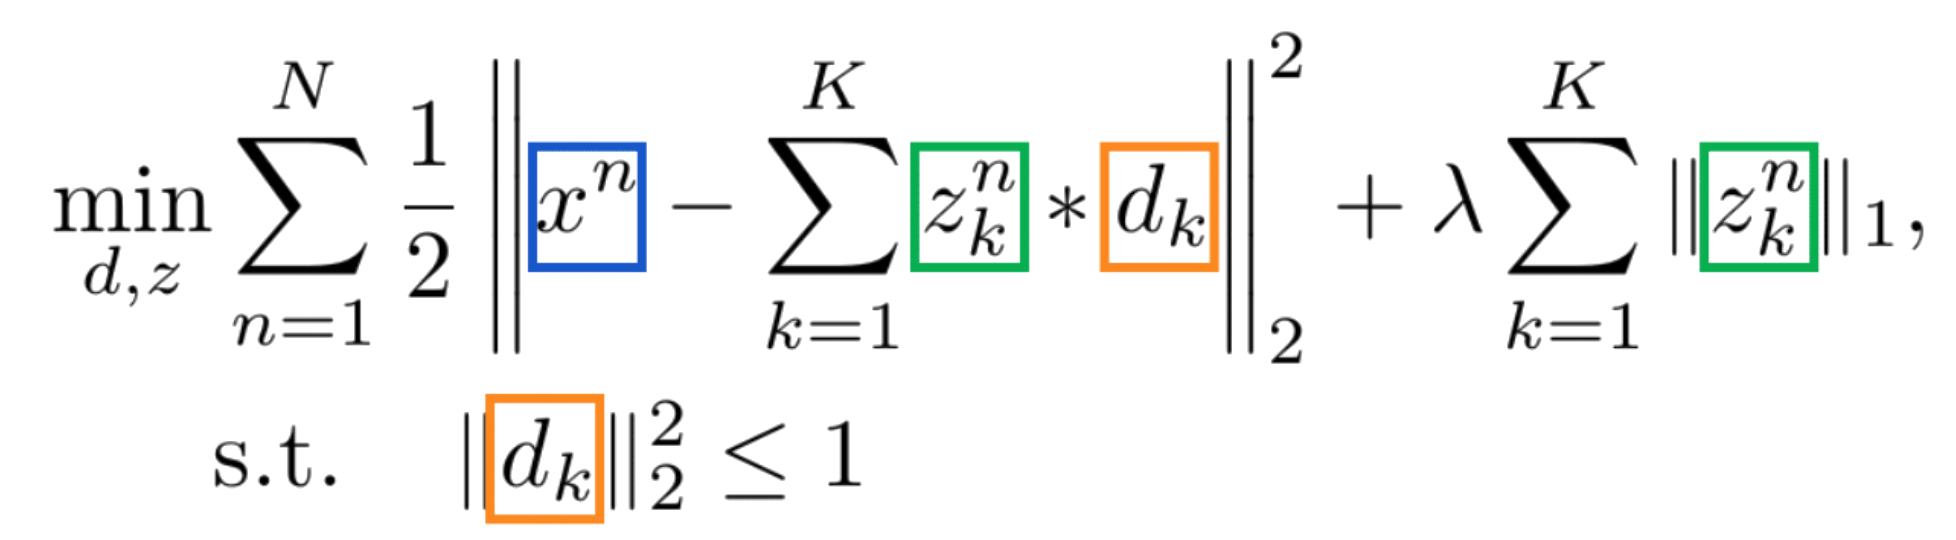
\includegraphics[width=\textwidth]{csc_eq_l1}
    \end{columns}
}
\end{frame}
\begin{frame}[t]
\frametitle{Notation}
    \textbf{Sparse Convolutional model:}
	\begin{align*}
		X[t] & = \sum_{k=1}^K (\pmb D_k*Z_k)[t] + \mathcal E[t]
	\end{align*}
	\vskip.5em
	with \makebox[1em]{$Z$} sparse. {\color{gray} Few of its coefficients are non-zero.}
    \vskip1em
    \begin{itemize}\itemsep1em
        \item $X$ is a signal of length $T$
        \item $\mathcal E$ is a noise signal of length $T$ 
        \item $\pmb D$ is a set of $K$ patterns of length $L$
        \item $Z$ is a signal of length $\widetilde{T} = T-L+1$ in $\Rset^K$ 
    \end{itemize}
\end{frame}

%------------------------------------------------------------------------
\subsection{Convolutional dictionary Learning}
%------------------------------------------------------------------------
\begin{frame}[t]
\frametitle{Convolutional Dictionary Learning}
Dictionary learning optimization problem for $\{X^{[n]}\}_{n=1}^N$ 
\[\hskip-2em\begin{split}
 \min_{Z, \|\pmb D_k\|\le 1}\frac{1}{N}\sum_{n=1}^N
			\underbrace{\| X^{[n]} - \sum_{k=1}^K\pmb D_k *  Z_k^{[n]}\|_2^2
						}_{E(Z) \text{ data fit}}
			+ \underbrace{\lambda\| Z^{[n]}\|_1
						}_{\text{penalization}}
\end{split}\]
with a regularization parameter $\lambda > 0$.\\[1.5em]
This problem is bi-convex and an approximate solution is obtained through \textbf{alternate minimization}. \mycite{Engan1999, Grosse2007}
\end{frame}

\begin{frame}[t]
\frametitle{$\pmb D$-step: Dictionary updates}
$\rightarrow Z$ fixed, update $\pmb D$
\[
	\pmb D^* = \argmin_{\|\pmb D_k\|_2 \le 1}\frac{1}{N}\sum_{n=1}^N
			\| X^{[n]} - \sum_{k=1}^K\pmb D_k *  Z_k^{[n]}\|_2^2
\]
\vskip1.5em
%
\underline{\textbf{Related Algorithms:}}\\[.5em]
\begin{itemize}\itemsep.5em
	\item Proximal Gradient Descent (PDG) \mycite{Rockafellar1976}
	\item Accelerated PGD \mycite{Nesterov1983}
	\item Block Coordinate Descent \mycite{Mairal2010}
	\item Alternated Direction Method of Multiplier (ADMM)\\\mycite{Gabay1976}
\end{itemize}
\end{frame}

\begin{frame}[t]
%\vskip-1em
\frametitle{$Z$-step: Convolutional Sparse Coding (CSC)}
$\rightarrow \pmb D$ fixed, update $Z$
\[
	Z^{[n],*} = \argmin_{Z^{[n]}}\| X^{[n]} - \sum_{k=1}^K\pmb D_k *  Z_k^{[n]}\|_2^2
			+ \lambda\| Z^{[n]}\|_1
\]
\strongpoint{Independent for each $n\in\llbracket1, N\rrbracket$}
\vskip1em
%
\underline{\textbf{Related Algorithms:}}\\[.5em]
\begin{itemize}%\itemsep.5em
	\item Iterative Soft-Thresholding Algorithm (ISTA)\\\mycite{Daubechies2004, Chalasani2013}
	\item Fast ISTA \\\mycite{Beck2009, Wohlberg2016}
	\item Alternated Direction Method of Multiplier (ADMM)\\\mycite{Gabay1976, Bristow2013}
	\item Coordinate Descent (CD) \\\mycite{Friedman2007, Kavukcuoglu2013}
\end{itemize}

	
\end{frame}

%\begin{frame}
%	\frametitle{Coordinate Descent \mycite{Friedman2007}}
%	{
%	\vskip2em
%	Select a coordinate $(k, t)$ and update it to the value
%	\[
%		Z_k'[t] = \argmin_{Z_k[t]}\| X - \sum_{k=1}^K\pmb D_k *  Z_k\|_2^2
%				+ \lambda\| Z\|_1
%	\]
%	with all other coordinates fixed.
	
%	\vskip2em
%	\centering
%	\inputTikZ{1}{cd_tikz}
%	}{ISTA \mycite{Daubechies2004}}{
%	\vskip2em
%	Proximal Gradient descent for Sparse Coding:
%	\[
%		Z^{(q+1)} = \text{Sh}\left(Z^{(q)} - \alpha\nabla E(Z^{(q)}), \alpha\lambda\right)
%	\]frametitle
%	with Sh$(Z_k[t], \lambda) = \text{sign}(Z_k[t])\max(|Z_k[t]|-\lambda, 0)$.

%	\vskip2em	
%	\centering
%	\inputTikZ{1}{pgd_tikz}
%	}
%\end{frame}


%%---------------------------------------------------------------------------
%\subsection{Accelerating the sparse coding}
%%---------------------------------------------------------------------------
%
%
%\begin{frame}{Part I: Adaptive Optimization}
%
%\vskip2em
%We have to solve $N$ independent problems with a common structure $\pmb D$,\\[.5em]
%\[
%Z^{[n],*} = \argmin_{Z^{[n]}}\| X^{[n]} - \sum_{k=1}^K\pmb D_k *  Z_k^{[n]}\|_2^2
%+ \lambda\| Z^{[n]}\|_1
%\]\vskip2em
%{\textbf{Can we use this structure to accelerate the resolution?}\\[1em]}
%\visible<2->{
%    Yes, with the Learned ISTA. \mycite{Gregor10}\\[1em]
%    %
%    \textbf{Why does it work?} \visible<3>{Analysis in the context of sparse coding.\\\hfill{\color{gray}(no convolution)}}\\
%}
%\end{frame}
%
%
%
%\begin{frame}
%\frametitle{Part II: Coordinate Descent for CSC}
%
%	Coordinate descent only performs local updates at each iteration.
%	\strongpoint{More efficient for convolutional model with long signals.}
%    \vskip2.5em
%    {\bf Can we improve it with the structure of our problem?}
%    \vskip1em
%    Improving CD efficiency for the convolutional structure:\\[1em]
%	\begin{itemize}\itemsep1em
%		\item Locally Greedy Coordinate Descent.
%		\item Asynchronous and distributed algorithms: DICOD and DiCoDiLe.
%	\end{itemize}
%
%
%\end{frame}
%
%
%
%\begin{frame}
%\frametitle{Part III: Rank-1 Contrained CDL}
%
%
%For electrophisiological signals, the CDL reads,
%\[\hskip-2em\begin{split}
%    \min_{Z, \pmb D}\frac{1}{N}\sum_{n=1}^N
%        \| X^{[n]} - \sum_{k=1}^K\pmb D_k *  Z_k^{[n]}\|_2^2
%+ \lambda\| Z^{[n]}\|_1 + \textbf{1}_{\Omega}(D)
%\end{split}\]
%
%\vskip1em
%However, this model does not account for the physics of the problem.\\[1em]
%
%Can we constrain the structure of the dictionary to learn more interpretable atoms?
%
%\strongpoint{Use rank-1 constraints to accomodate Maxwell's equations.}
%
%
%\end{frame}
%
%


\biblio{}
\end{document}